\documentclass[journal,a4paper,onecolumn]{IEEEtran}

% *** GRAPHICS RELATED PACKAGES ***
%
\ifCLASSINFOpdf
   \usepackage[pdftex]{graphicx}
  % declare the path(s) where your graphic files are
   \graphicspath{{./pdf/}{./jpeg/}}
  % and their extensions so you won't have to specify these with
  % every instance of \includegraphics
   \DeclareGraphicsExtensions{.pdf,.jpeg,.png}
\else
  % or other class option (dvipsone, dvipdf, if not using dvips). graphicx
  % will default to the driver specified in the system graphics.cfg if no
  % driver is specified.
   \usepackage[dvips]{graphicx}
  % declare the path(s) where your graphic files are
   \graphicspath{{./eps/}}
  % and their extensions so you won't have to specify these with
  % every instance of \includegraphics
   \DeclareGraphicsExtensions{.eps}
\fi

\usepackage{amsmath}
\usepackage{hyperref}
\hypersetup{
	colorlinks,
	urlcolor=blue,
	citecolor=black}

% correct bad hyphenation here
\hyphenation{op-tical net-works semi-conduc-tor}

\begin{document}
\addtocounter{page}{1}
% paper title
% can use linebreaks \\ within to get better formatting as desired
\title{~\vskip -5mm Recursive Types and their Properties}
%
%
% author names and IEEE memberships
% note positions of commas and nonbreaking spaces ( ~ ) LaTeX will not break
% a structure at a ~ so this keeps an author's name from being broken across
% two lines.
% use \thanks{} to gain access to the first footnote area
% a separate \thanks must be used for each paragraph as LaTeX2e's \thanks
% was not built to handle multiple paragraphs

\author{\textit{\begin{Large}\textsuperscript{1}Michal~SAKM\'{A}R, \textsuperscript{2}Gabriel~BUG\'{A}R\end{Large}}\\
\bigskip
\textsuperscript{1}Department of Electronics and Multimedia Communications, Faculty of Electrical Engineering and Informatics Technical University of Ko\v{s}ice, Slovak Republic\\
\textsuperscript{2}Department of Cybernetics and Artificial Intelligence, Faculty of Electrical Engineering and Informatics Technical University of Ko\v{s}ice, Slovak Republic\\
\bigskip
\textsuperscript{1}michal.sakmar@tuke.sk, \textsuperscript{2}gabriel.bugar@tuke.sk}

% make the title area
\maketitle

\begin{abstract}
\textbf{\textit{Abstract}}~\textendash~\bfseries
These instructions give you guidelines for preparing papers for scientific conferences. Use this document as a template if you are using \LaTeXe. Otherwise, use this document as an instruction set. Define all symbols used in the abstract. Do not cite references in the abstract.
\end{abstract}

% Note that keywords are not normally used for peerreview papers.
\begin{IEEEkeywords}
\textbf{\textit{Keywords}}~\textendash~\bfseries
About four key words or phrases in alphabetical order, separated by commas
\end{IEEEkeywords}

% For peerreview papers, this IEEEtran command inserts a page break and
% creates the second title. It will be ignored for other modes.
%\IEEEpeerreviewmaketitle

\section{Introduction}

This document is a template for \LaTeX. \textbf{Do not change the font sizes or line spacing to squeeze more text into a limited number of pages.} Use italics for emphasis; do not underline.

\section{Procedure for Paper Submission}

\subsection{Figures}

Format and save your graphic images using a suitable graphics processing program that will allow you to create the images as PostScript (PS), Encapsulated PostScript (EPS), or Tagged Image File Format (TIFF), sizes them, and adjusts the resolution settings. If you created your source files in one of the following you will be able to submit the graphics without converting to a PS, EPS, or TIFF file: Microsoft Word, Microsoft PowerPoint, Microsoft Excel, or Portable Document Format (PDF).

\subsection{Electronic Image Files (Optional)}

Import your source files in one of the following: Microsoft Word, Microsoft PowerPoint, Microsoft Excel, or Portable Document Format (PDF); you will be able to submit the graphics without converting to a PS, EPS, or TIFF files. Image quality is very important to how yours graphics will reproduce. Even though we can accept graphics in many formats, we cannot improve your graphics if they are poor quality when we receive them. If your graphic looks low in quality on your printer or monitor, please keep in mind that cannot improve the quality after submission.

If you are preparing images in TIFF, EPS, or PS format, note the following. High-contrast line figures and tables should be prepared with 600 dpi resolution and saved with no compression, 1 bit per pixel (monochrome), with file names in the form of ``fig3.tif'' or ``table1.tif.''

Photographs and grayscale figures should be prepared with 300 dpi resolution and saved with no compression, 8 bits per pixel (grayscale).

\subsection*{Sizing of Graphics}

Most charts graphs and tables are one column wide (3 1/2 inches or 21 picas) or two-column width (7 1/16 inches, 43 picas wide). We recommend that you avoid sizing figures less than one column wide, as extreme enlargements may distort your images and result in poor reproduction. Therefore, it is better if the image is slightly larger, as a minor reduction in size should not have an adverse affect the quality of the image.

\subsection*{How to create a PostScript File}

First, download a PostScript printer driver from \url{http://www.adobe.com/support/downloads/pdrvwin.htm} (for Windows) or from \url{http://www.adobe.com/support/downloads/}\\\url{pdrvmac.htm} (for Macintosh) and install the ``Generic PostScript Printer'' definition. Print to a file using the PostScript printer driver. File names should be of the form ``fig5.ps.'' Use Open Type fonts when creating your figures, if possible. A listing of the acceptable fonts are as follows: Open Type Fonts: Times Roman, Helvetica, Helvetica Narrow, Courier, Symbol, Palatino, Avant Garde, Bookman, Zapf Chancery, Zapf Dingbats, and New Century Schoolbook.

\section{Math}

If you are using Word, use either the Microsoft Equation Editor or the MathType add-on (\url{http://www.mathtype.com}) for equations in your paper (Insert | Object | Create New | Microsoft Equation or MathType Equation). “Float over text” should not be selected.

\section{Helpful Hints}

\begin{figure}[!t]
	\centering
	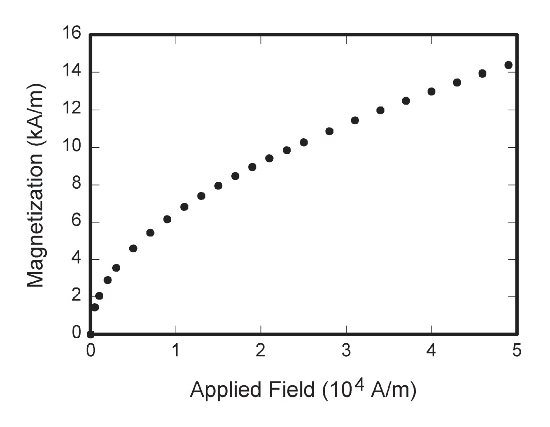
\includegraphics[width=0.95\columnwidth]{./eps/fig1}
% where an .eps filename suffix will be assumed under latex, 
% and a .pdf suffix will be assumed for pdflatex; or what has been declared
% via \DeclareGraphicsExtensions.
	\caption{Magnetization as a function of applied field. Note that ``Fig.'' is abbreviated.}
	\label{fig_sim}
\end{figure}

% An example of a double column floating figure using two subfigures.
% (The subfig.sty package must be loaded for this to work.)
% The subfigure \label commands are set within each subfloat command, the
% \label for the overall figure must come after \caption.
% \hfil must be used as a separator to get equal spacing.
% The subfigure.sty package works much the same way, except \subfigure is
% used instead of \subfloat.
%
%\begin{figure*}[!t]
%\centerline{\subfloat[Case I]\includegraphics[width=2.5in]{subfigcase1}%
%\label{fig_first_case}}
%\hfil
%\subfloat[Case II]{\includegraphics[width=2.5in]{subfigcase2}%
%\label{fig_second_case}}}
%\caption{Simulation results}
%\label{fig_sim}
%\end{figure*}

\subsection{Figures and Tables}

All figures, figure captions, and tables can be at the end of the paper. Large figures and tables may span both columns. Place figure captions below the figures; place table titles above the tables. If your figure has two parts, include the labels ``(a)'' and ``(b)'' as part of the artwork. Please verify that the figures and tables you mention in the text actually exist. \textbf{Please do not include captions as part of the figures. Do not put captions in ``text boxes'' linked to the figures. Do not put borders around the outside of your figures.} Use the abbreviation ``Fig.'' even at the beginning of a sentence. Do not abbreviate ``Table.'' Tables are numbered with Roman numerals.

Figure axis labels are often a source of confusion. Use words rather than symbols. As an example, write the quantity ``Magnetization,'” or ``Magnetization $M$,'' not just ``$M$.'' Put units in parentheses. Do not label axes only with units. As in Fig. 1, for example, write ``Magnetization ($A/m$)'' or ``Magnetization ($A.m^{-1}$),'' not just ``$A/m$.'' Do not label axes with a ratio of quantities and units. For example, write ``Temperature ($^{\circ} C$),'' not ``Temperature/$^{\circ} C$.''

Multipliers can be especially confusing. Write ``Magnetization ($kA/m$)'' or ``Magnetization ($10^{3} A/m$).'' Do not write ``Magnetization ($A/m$) $\times$ 1000'' because the reader would not know whether the top axis label in Fig. 1 meant 16000 $A/m$ or 0.016 $A/m$. Figure labels should be legible, approximately 8 to 12 point type.

\subsection{References}

Number citations consecutively in square brackets \cite{Calvetti}. The sentence punctuation follows the brackets \cite{Pan}. Multiple references \cite{Pan}, \cite{Pan} are each numbered with separate brackets [1]–[3]. Do not use ``Ref. [3]'' or ``reference [3]'' except at the beginning of a sentence: ``Reference [3] shows ... .''

Please note that the references at the end of this document are in the preferred referencing style. Give all authors’ names; do not use ``et al.'' unless there are six authors or more. Use a space after authors’ initials. Papers that have not been published should be cited as ``unpublished'' \cite{Johansson}. Papers that have been accepted for publication, but not yet specified for an issue should be cited as ``to be published'' [6]. Papers that have been submitted for publication should be cited as ``submitted for publication'' [6].

Capitalize only the first word in a paper title, except for proper nouns and element symbols. For papers published in translation journals, please give the English citation first, followed by the original foreign-language citation [8].

\begin{table}[!t]
	\renewcommand{\arraystretch}{1.3}
	\caption{Units for Magnetic Properties}
	\label{table_example}
	\centering
	\begin{tabular}{lll}
		\hline\hline
		Symbol & Quantity & Conversion from Gaussian and\\
		& &  CGS EMU to SI$^a$ \\
		\hline
		$\Phi$ & magnetic flux & $1 Mx\rightarrow10^{-8}Wb=10^{-8}Vs$\\
		$B$ & magnetic induction & $1 G\rightarrow10^{-4}T=10^{-4}Wb/m^2$ \\
		$H$ & magnetic field strength & $1 Oe\rightarrow10^3/(4\pi)A/m$ \\
		\hline\hline
		\multicolumn{3}{p{0.95\columnwidth}}{Vertical lines are optional in tables. Statements that serve as captions for the entire table do not need footnote letters.}\\
		\multicolumn{3}{p{0.95\columnwidth}}{$^a$Gaussian units are the same as cgs emu for magnetostatics; Mx = maxwell, G = gauss, Oe = oersted; Wb = weber, V = volt, s = second, T = tesla, m = meter, A = ampere, J = joule, kg = kilogram, H = henry.}
	\end{tabular}
\end{table}

\subsection{Abbreviations and Acronyms}

Define abbreviations and acronyms the first time they are used in the text, even after they have already been defined in the abstract. Abbreviations such as IEEE, SI, ac, and dc do not have to be defined. Abbreviations that incorporate periods should not have spaces: write ``C.N.R.S.,'' not ``C. N. R. S.'' Do not use abbreviations in the title unless they are unavoidable (for example, ``IEEE'').

\subsection{Equations}

Number equations consecutively with equation numbers in parentheses flush with the right margin, as in (1). First use the equation editor to create the equation. Then select the ``Equation'' markup style. Press the tab key and write the equation number in parentheses. To make your equations more compact, you may use the solidus ( / ), the exp function, or appropriate exponents. Use parentheses to avoid ambiguities in denominators. Punctuate equations when they are part of a sentence, as in

\begin{equation}
	\begin{split}
		\int_{0}^{r_2}F(r,\varphi)dr d\varphi=[\sigma r_2/(2\mu _0)]\cdot \\ \cdot\int_{0}^{\infty}exp(-\lambda|z_j-z_i)\lambda^{-1}J_1(\lambda r_2)J_0(\lambda r_i)d\lambda
	\end{split}
\end{equation}


Be sure that the symbols in your equation have been defined before the equation appears or immediately following. Italicize symbols (T might refer to temperature, but T is the unit tesla). Refer to ``(1),'' not ``Eq. (1)'' or ``equation (1),'' except at the beginning of a sentence: ``Equation (1) is ... .''

\subsection{Other Recommendations}

Use one space after periods and colons. Hyphenate complex modifiers: ``zero-field-cooled magnetization.'' Avoid dangling participles, such as, ``Using (1), the potential was calculated.'' [It is not clear who or what used (1).] Write instead, ``The potential was calculated by using (1),'' or ``Using (1), we calculated the potential.''

Use a zero before decimal points: ``0.25,'' not ``.25.'' Use ``$cm^3$,'' not ``cc.'' Indicate sample dimensions as ``$0.1 cm \times 0.2 cm$,'' not ``$0.1 \times 0.2 cm^2$.'' The abbreviation for ``seconds'' is ``s,'' not ``sec.'' Do not mix complete spellings and abbreviations of units: use ``$Wb/m^2$'' or ``webers per square meter,'' not ``webers/$m^2$.'' When expressing a range of values, write ``7 to 9'' or ``7-9,'' not ``7\~9.''

A parenthetical statement at the end of a sentence is punctuated outside of the closing parenthesis (like this). (A parenthetical sentence is punctuated within the parentheses.) In American English, periods and commas are within quotation marks, like ``this period.'' Other punctuation is ``outside''! Avoid contractions; for example, write ``do not'' instead of ``don’t.'' The serial comma is preferred: ``A, B, and C'' instead of ``A, B and C.''

If you wish, you may write in the first person singular or plural and use the active voice (``I observed that ...'' or ``We observed that ...'' instead of ``It was observed that ...''). Remember to check spelling. If your native language is not English, please get a native English-speaking colleague to carefully proofread your paper.

\section{Some Common Mistakes}

The word ``data'' is plural, not singular. The subscript for the permeability of vacuum $\mu 0$ is zero, not a lowercase letter ``o.'' The term for residual magnetization is ``remanence''; the adjective is ``remanent''; do not write ``remnance'' or ``remnant.'' Use the word ``micrometer'' instead of ``micron.'' A graph within a graph is an ``inset,'' not an ``insert.'' The word ``alternatively'' is preferred to the word ``alternately'' (unless you really mean something that alternates). Use the word ``whereas'' instead of ``while'' (unless you are referring to simultaneous events). Do not use the word ``essentially'' to mean ``approximately'' or ``effectively.'' Do not use the word ``issue'' as a euphemism for ``problem.'' When compositions are not specified, separate chemical symbols by en-dashes; for example, ``NiMn'' indicates the intermetallic compound $Ni_{0.5}Mn_{0.5}$ whereas ``Ni–Mn'' indicates an alloy of some composition $Ni_xMn_{1-x}$.

Prefixes such as ``non,'' ``sub,'' ``micro,'' ``multi,'' and ``ultra'' are not independent words; they should be joined to the words they modify, usually without a hyphen. There is no period after the ``et'' in the Latin abbreviation ``et al.'' (it is also italicized). The abbreviation ``i.e.,'' means ``that is,'' and the abbreviation ``e.g.,'' means ``for example'' (these abbreviations are not italicized).
An excellent style manual and source of information for science writers is [9]. A general IEEE style guide and an Information for Authors are both available at \url{http://www.ieee.org/web/publications/authors/transjnl}

\section{Conclusion}

A conclusion section is not required. Although a conclusion may review the main points of the paper, do not replicate the abstract as the conclusion. A conclusion might elaborate on the importance of the work or suggest applications and extensions.

% if have a single appendix:
%\appendix[Proof of the Zonklar Equations]
% or
%\appendix  % for no appendix heading
% do not use \section anymore after \appendix, only \section*
% is possibly needed

% use appendices with more than one appendix
% then use \section to start each appendix
% you must declare a \section before using any
% \subsection or using \label (\appendices by itself
% starts a section numbered zero.)
%

% you can choose not to have a title for an appendix
% if you want by leaving the argument blank
\appendices
\section{}
Appendixes, if needed, appear before the acknowledgment.

% use section* for acknowledgement
\section*{Acknowledgment}

The preferred spelling of the word ``acknowledgment'' in American English is without an ``e'' after the ``g.'' Use the singular heading even if you have many acknowledgments. Avoid expressions such as ``One of us (S.B.A.) would like to thank ... .'' Instead, write ``F. A. Author thanks ... .''

% Can use something like this to put references on a page
% by themselves when using endfloat and the captionsoff option.
%\ifCLASSOPTIONcaptionsoff
%  \newpage
%\fi

% trigger a \newpage just before the given reference
% number - used to balance the columns on the last page
% adjust value as needed - may need to be readjusted if
% the document is modified later
%\IEEEtriggeratref{8}
% The "triggered" command can be changed if desired:
%\IEEEtriggercmd{\enlargethispage{-5in}}

% references section

% can use a bibliography generated by BibTeX as a .bbl file
% BibTeX documentation can be easily obtained at:
% http://www.ctan.org/tex-archive/biblio/bibtex/contrib/doc/
% The IEEEtran BibTeX style support page is at:
% http://www.michaelshell.org/tex/ieeetran/bibtex/
\bibliographystyle{IEEEtran}
% argument is your BibTeX string definitions and bibliography database(s)
\bibliography{bibliography}

\end{document}
